% The packages used here are just a sample. You may need others, and may not need some of these. It doesn't hurt to leave them in, unless they start to conflict with other packages you've added. Chapter 2 has example code for equations, figures, tables, citations, abbreviations, etc. If there are sections labeled 'optional' that you don't want, just comment them out. -jg

\documentclass[reqno,12pt,oneside]{report} % right-side equation numbering, 12 point font, print one-sided
%\documentclass[reqno,12pt,twoside,openright]{report} % right-side equation numbering, 12 point font, print two-sided, Chapters start on odd pages. Rackham only accepts one-sided, so this is for personal printings.

\usepackage{rac}         % Use Rackham thesis style file
\usepackage{aas_macros}  % To allow the reading of ADS journal references in the bibliography
\usepackage[intlimits]{amsmath} % Puts the limits of integrals on top and bottom
\usepackage{amsxtra}     % Use various AMS packages
\usepackage{amsthm}
\usepackage{amssymb}
\usepackage{amsfonts}
\usepackage{graphicx}    % Add some packages for figures. Read epslatex.pdf on ctan.tug.org
\usepackage{rotating}
\usepackage{color}
\usepackage{mdframed}
\usepackage{epsfig}
\usepackage{subfigure}   % To make subfigures. Read subfigure.pdf on ctan.tug.org
\usepackage{verbatim}
\usepackage{natbib}      % Allows you to use BibTeX
\usepackage{acronym} % For the List of Abbreviations. Read acronym.pdf on ctan.tug.org
\usepackage{setspace}
\usepackage[ruled]{algorithm2e}
%\usepackage[acronym]{glossaries}
\usepackage{nomencl}
%\usepackage{biblatex}
%\addbibresource{References.bib}

\usepackage[nottoc,notlof,notlot]{tocbibind}
\renewcommand\bibname{References}

\makenomenclature
  % Allows you to specify the line spacing
%\doublespacing           % \onehalfspacing for 1.5 spacing, \doublespacing for 2.0 spacing.
\newcommand{\sun}{\ensuremath{\odot}} % sun symbol is \sun
%%%%%%%%%%%%%%%%%%%%%%%%%%%%%%%%%%%%%%%%%%%%%%%%%%%%%%%%%%%%%%%%%%%%%%%%%%%%%%%

% Various theorem environments. All of the following have the same numbering
% system as theorem.

\theoremstyle{plain}
\newtheorem{theorem}{Theorem}
\newtheorem{prop}[theorem]{Proposition}
\newtheorem{corollary}[theorem]{Corollary}
\newtheorem{lemma}[theorem]{Lemma}
\newtheorem{question}[theorem]{Question}
\newtheorem{conjecture}[theorem]{Conjecture}
\newtheorem{assumption}[theorem]{Assumption}

\theoremstyle{definition}
\newtheorem{definition}[theorem]{Definition}
\newtheorem{notation}[theorem]{Notation}
\newtheorem{condition}[theorem]{Condition}
\newtheorem{example}[theorem]{Example}
\newtheorem{introduction}[theorem]{Introduction}

\theoremstyle{remark}
\newtheorem{remark}[theorem]{Remark}
%%%%%%%%%%%%%%%%%%%%%%%%%%%%%%%%%%%%%%%%%%%%%%%%%%%%%%%%%%%%%%%%%%%%%%%%%%%%%%%

\numberwithin{theorem}{chapter}     % Numbers theorems "x.y" where x
                                    % is the section number, y is the
                                    % theorem number

%\renewcommand{\thetheorem}{\arabic{chapter}.\arabic{theorem}}

%\makeatletter                      % This sequence of commands will
%\let\c@equation\c@theorem          % incorporate equation numbering
%\makeatother                       % into the theorem numbering scheme

%\renewcommand{\theenumi}{(\roman{enumi})}

%%%%%%%%%%%%%%%%%%%%%%%%%%%%%%%%%%%%%%%%%%%%%%%%%%%%%%%%%%%%%%%%%%%%%%%%%%%%%%

% If printing two-sided, this makes sure that any blank page at the
% end of a chapter will not have a page number.
\makeatletter
\def\cleardoublepage{\clearpage\if@twoside \ifodd\c@page\else
\hbox{}
\thispagestyle{empty}
\newpage
\if@twocolumn\hbox{}\newpage\fi\fi\fi}
\makeatother

%%%%%%%%%%%%%%%%%%%%%%%%%%%%%%%%%%%%%%%%%%%%%%%%%%%%%%%%%%%%%%%%%%%%%%%%%%%%%%

%This command creates a box marked ``To Do'' around text.
%To use type \todo{  insert text here  }.

\newcommand{\todo}[1]{\vspace{5 mm}\par \noindent
\marginpar{\textsc{To Do}}
\framebox{\begin{minipage}[c]{0.95 \textwidth}
\tt\begin{center} #1 \end{center}\end{minipage}}\vspace{5 mm}\par}



%%\usepackage[refpage]{nomencl}
%%\renewcommand{\nomname}{List of Notations}
%%\renewcommand*{\pagedeclaration}[1]{\unskip\dotfill\hyperpage{#1}}
%%\makenomenclature
%%
%%
%%\usepackage{makeidx}
%%\makeindex
%%

% Please add the following required packages to your document preamble:
\usepackage{multirow}
\usepackage[table,xcdraw]{xcolor}
% If you use beamer only pass "xcolor=table" option, i.e. \documentclass[xcolor=table]{beamer}
\usepackage[normalem]{ulem}
\useunder{\uline}{\ul}{}

%%%%%%%%%%%%%%%%%%%%%%%%%%%%%%%%%%%%%%%%%%%%%%%%%%%%%%%%%%%%%%%%%%%%%%%%%%%%%%%
\begin{document}

\bibliographystyle{plain}    % Set the bibliography style. agu04, plain, alpha, etc.
% Title page as required by Rackham dissertation guidelines
\titlepage{Activity based new technique of Effort \& Cost Estimation using Functional Measurement Type for web application. }{Sayed Mohsin Reza (Roll: 150102)}{Masters of Science}
{Electronics and Communication Engineering}{June, 2016}
{Dr. M. Shamim Kaiser}

% Begin the front matter as required by Rackham dissertation guidelines
\initializefrontsections

% Optional Frontispiece
%\frontispiece{
\includegraphics[width=6in]{Intro/Happy} Find a cool picture to go here.}

% Optional, but recommended, Copyright page
%\copyrightpage{Your Name}

% Page numbering. If you don't include a frontispiece or copyright page, you'll need to change this for two-sided printing.
\makeatletter
\if@twoside \setcounter{page}{4} \else \setcounter{page}{1} \fi
\makeatother

% Optional Dedication page
%\dedicationpage{To Our Beloved Parents}


%Optional declaration page
\startdeclarationpage
We hereby declare that this system is based on the results found by ourselves. Materials of work found by other are mentioned by reference. This system, neither in whole nor in part, has been previously submitted for any degree.

\bigskip
\bigskip
\bigskip


\begin{tabular}{p{5cm}p{5cm}p{5cm}}
\centering
  % after \\: \hline or \cline{col1-col2} \cline{col3-col4} ...
     &  &   \\
  Sayed  Mohsin  Reza &   & \\
  Roll: 150102 &    & \\

\end{tabular}




\label{declaration}


%Optional Certificate page
\startcertificatepage

This is to certify that the thesis proposal entitled \textbf{Activity based new technique of Effort \& Cost Estimation using Functional Measurement Type for web application} and submitted by Sayed Mohsin Reza for the degree of Master's of Science. He embodies original work under my supervision to the best of my knowledge.

\bigskip
\bigskip
\bigskip
\bigskip
\bigskip
\bigskip

  % after \\: \hline or \cline{col1-col2} \cline{col3-col4} ...
\noindent (Signature in full of
The Supervisor)
 \\
  Dr. M Shamim Kaiser \\ Associate Professor,  \\
  Institute of Information Technology,\\
  Jahangirnagar University.\\


\label{Certificate}







% Optional Acknowledgements page
\startacknowledgementspage

First of all we would like to thank the Almighty for giving us the opportunity to complete this work successfully. Our acknowledgement is meant to express our sincere gratitude to all those people who have been associated with this thesis and have helped us with it and by sharing their opinions and experiences through which we received the required information crucial for our system. We are thankful to our parents for their relentless support. Most importantly we are tremendously grateful to our honorable supervisor who took time out of his hectic schedule to guide us and provide us with all the necessary materials and sufficient knowledge that was the major requirement. Finally, we express our thanks to our honourable teacher Dr. M. Shamim Kaiser for giving us the opportunity to learn the subject in a practical approach.

\label{Acknowledgements}

%Optional Abstract page
\startabstractpage
Software cost models and effort approximations support project supervisors to distribute resources, control budgets
and agenda and develop modern practices, leading to projects completed on time and within financial plan. If cost and effort are determined suspicious in software projects, suitable occasions can be missed; whereas expectant predictions can be affected to some resource losing. In the context of web development, these issues are also vital, and very challenging given that web projects have short schedules and very fluidic opportunity. Since software projects are continually changed in nature, earlier projects may not necessarily cover all aspects of a new project when used
as a basis for cost estimation. Preliminary software estimation models are constructed on regression analysis or mathematical sources. This paper aims to propose an approach to develop the correctness of software effort and cost estimation using the structure of data set of a web application. All the measures collected, apart from total effort, were introduced using the original web hypermedia applications to ensure that functional measurement types were precisely measured. 
\label{Abstract}

% Optional Preface page
%\startprefacepage
%\input{Preface}
%\label{Preface}

% Table of contents, list of , etc.
\tableofcontents     % Required
\listoffigures       % Required if there is more than one figure
\listoftables        % Required if there is more than one table
%%%%%%%%%%%%%%%%%%%\printnomenclature

%\listofmaps          % Required if there is more than one map
%\listofappendices    % Required if there is more than one appendix
%%%%----------------------------------------------------------------------------------------
%%%%	SYMBOLS
%%%%----------------------------------------------------------------------------------------
%%%
%%%%\clearpage % Start a new page
%%%%
%%%%\lhead{\emph{Symbols}} % Set the left side page header to "Symbols"
%%%
%%%\listofnomenclature{lll} % Include a list of Symbols (a three column table)
%%%{
%%%$a$ & distance & m \\
%%%$P$ & power & W (Js$^{-1}$) \\
%%%% Symbol & Name & Unit \\
%%%
%%%& & \\ % Gap to separate the Roman symbols from the Greek
%%%
%%%$\omega$ & angular frequency & rads$^{-1}$ \\
%%%% Symbol & Name & Unit \\
%%%}

\listofabbreviations % Optional. Abbreviations should be stored in a file named abbr.tex
% Optional in-dissertation Abstract Page
%\startabstractpage
%{The Title of Your Dissertation}{Your Name}{Chair: Albert Einstein}
%Software cost models and effort approximations support project supervisors to distribute resources, control budgets
and agenda and develop modern practices, leading to projects completed on time and within financial plan. If cost and effort are determined suspicious in software projects, suitable occasions can be missed; whereas expectant predictions can be affected to some resource losing. In the context of web development, these issues are also vital, and very challenging given that web projects have short schedules and very fluidic opportunity. Since software projects are continually changed in nature, earlier projects may not necessarily cover all aspects of a new project when used
as a basis for cost estimation. Preliminary software estimation models are constructed on regression analysis or mathematical sources. This paper aims to propose an approach to develop the correctness of software effort and cost estimation using the structure of data set of a web application. All the measures collected, apart from total effort, were introduced using the original web hypermedia applications to ensure that functional measurement types were precisely measured. 
%\label{Abstract}

\startthechapters
% The individual files for each of the chapters are put here.
% Save each chapter of your thesis to a seperate tex file
% and then use the \input command to include this file in your
% thesis.  For instance you can save a file to "intro.tex" and
% then type \input{intro}.

 %\chapter{Introduction}
 \label{chap:Intro}
 \chapter{Introduction}
%\label{chap:GettingStarted}

\section{Introduction}
%\label{sec:ChoosingAdvisor}
Software cost models and effort approximations support project supervisors to distribute resources, control budgets and agenda and develop modern practices, leading to projects completed on time and within financial plan. If cost and effort are determined suspicious in software projects, suitable occasions can be missed; whereas expectant predictions can be affected to some resource losing. In the context of web development, these issues are also vital and very challenging given that web projects have short schedules and very fluidic opportunity. Since software projects are continually changed in nature, earlier projects may not necessarily cover all aspects of a new project when used as a basis for cost estimation. Preliminary software estimation models are constructed on regression analysis or mathematical sources.
\section{System Review}

In this arena, some applications are run sequentially. Some of them are – OpenConf, OCS,EasyChair,CMT etc.Some
Modules of this System: Acceptance,Bidding,Discussion
Form Fields,CAPTCHA,File Type, Proceedings.\newline
\textbf{OpenConf:}Install system, check configuration and enable modules, open submission,
 upload and reviewer signup, assign reviewers and advocates, decision and notification.\cite{ref2}\newline
In OpenConf,there has no support to create multi-conference system,payment method
,Website creation,A/R paper download option,speaker scheduling.\newline

\textbf{OCS(Open Conference System):} Open Conference Systems (OCS) is a free Web publishing tool that will create a complete Web presence for your scholarly conference.OCS will allow you to:create a conference web site,compose and send a call for papers,electronically accept paper and abstract submissions,allow paper submitters to edit their work,post conference proceedings and papers in a searchable format,post,if you wish,the original data sets,register participants,integrate post-conference online discussions.\cite{ref3}\newline
In OCS, there has no support to create IEEE eCopyright,Website creation,A/R paper download option,sponsor tracking and speaker scheduling.\newline
\textbf{CMT: Microsoft’s Academic Conference Management Service-} The Conference Management Toolkit (CMT) is a free conference management service sponsored by Microsoft Research.CMT is capable of handling the complex workflow of an academic conference including:Customizable paper submission, reviewer,and author feedback forms,Author notification,Review submission etc.\cite{ref6}\newline
In CMT, there has no support to create multi-conference system,support multiple paper submission in one account,payment method,Website creation,A/R paper download option.\newline
\textbf{EasyChair:} EasyChair is a conference management system that is flexible, easy to use, and has many features to make it suitable for various conference models\cite{ref4}\newline
In EasyChair, there has no support to create multi-conference system,IEEE eCopyright,payment method,Website creation,A/R paper download option.\newline
Comparison above all systems with ProConf according to free addition.Such as:\newline

\begin{center}
\begin{table}[htbp]
   \begin{tabular}{|c|c|c|c|c|c|}
     \hline
     % after \\: \hline or \cline{col1-col2} \cline{col3-col4} ...
     Topics & ProConf & OpenConf & OCS & EasyChair & CMT \\\hline
     Make Submission & Y & Y & Y & Y & Y \\\hline
     Allow Multiconference & Y & N & Y & Y & N\\\hline
     Payment System & Y &N & Y & N & N  \\\hline
     Create Website  & Y & N & Y & N & N \\\hline
     P/N Author Registration & Y & Y & N & N & N \\\hline
     IEEE eCopyright & Y & N & N & N & Y \\\hline
     A/R paper Download option & Y & N & N & N & N\\\hline
     Program  Schedule Creation & Y &N & N & N & N \\\hline
     Online Registration & Y & Y & Y & y & Y\\\hline
     Speaker scheduling & Y & N & N & N & N\\\hline
     Multi-track support & Y & N & N & Y & N\\\hline
     MPS in one account & Y & N & N & N& N\\\hline
     Track Assign       &Y &N &N &Y &N \\\hline
     PM with RFID & Y & N & N & N & N\\\hline



   \end{tabular}
   \caption[Comparison with Existing System.]{Comparison with Existing System}
	\label{tab:comparison}

  \end{table}
  \end{center}


\section{Proposed  System }
Identify these problems, this proposed system target is to overcome those problems. Primarily, The Proposal entitled as ProConf can do Peer-Review, Abstract and Conference Management.ProConf is a free Web publishing tool that will create a complete Web presence for scholarly conference.
Proconf covers all aspects of online conference management and publishing, from setting up conference website to operational tasks such as submitting, reviewing, editing, publishing, archiving, and indexing of the conference papers.
Proconf also helps to manage the people involved in organizing a conference, reviewers, and authors,notifying readers and registrants, and assisting with the correspondence. Additionally, Payment system module is added and free as open source to anyone. In existing all conference system there has no concept of RFID. Main featured of proposed system is helpful to program management with RFID technologies.\newline
Below, there is an overview of the process ProConf uses.
\begin{center}
\begin{table}[htbp]
   \begin{tabular}{|c|c|c|c|c|c|}
     \hline
     % after \\: \hline or \cline{col1-col2} \cline{col3-col4} ...
     Topics &Chair &TC/C-C/M &Author & Reviewer & P/N \\\hline
     Install and Config &Y & N & N &N &N \\\hline
     Create Website & Y & N & N &N &N \\\hline
     Open and Close Submissions& Y & N & N &N &N \\\hline
     Sign-Up & N & Y & Y &Y &Y \\\hline
     Decision  and Notification & Y & N & N &N &N \\\hline
     CCPM & Y & N & N &N &N \\\hline
     Assign  Reviewers & Y & Y & N & N & N \\\hline
     OCRS & Y & N & N & N & N \\\hline
     Review Submission & N & Y & N & Y & N \\\hline
     PM with RFID  & Y & N & N & N & N \\\hline
     Give Comment after review  & N & TC-Y & N & N & N \\\hline
   \end{tabular}
   \caption[Proposed System Process.]{Proposed System Process}
	\label{tab:system process}

  \end{table}
  \end{center}







\section{System overview}
 ProConf is an open source multi-conference system to manage and publish online conferences. ProConf shields all aspects of available conference management and publishing, from setting up conference website to operational tasks such as submitting, reviewing, editing, publishing, archiving, and indexing of the conference papers. ProConf also helps to manage the people involved in organizing a conference, reviewers and authors, notifying readers and registered participants and assisting with the correspondence. Program Schedule, Conference Paper publish, Conference website development, Payment module etc are the main feature of this proposal. It has been designed to shrink the time and energy fanatical to the secretarial and executive tasks related with supervision of a online conference, while refining the record-keeping and efficiency of editorial processes.\newline
Additionally, ProConf is flexible and scalable. A single installation of ProConf can support the operation of multiple conferences, and multiple years for each conference. Each conference has its own unique URL as well as its own look and feel. ProConf can enable a single director to manage all aspects of a conference. At last, it is an open source helpline for anyone who conduct any online conference.


\begin{figure}[h!]
\centering
  % Requires \usepackage{graphicx}
  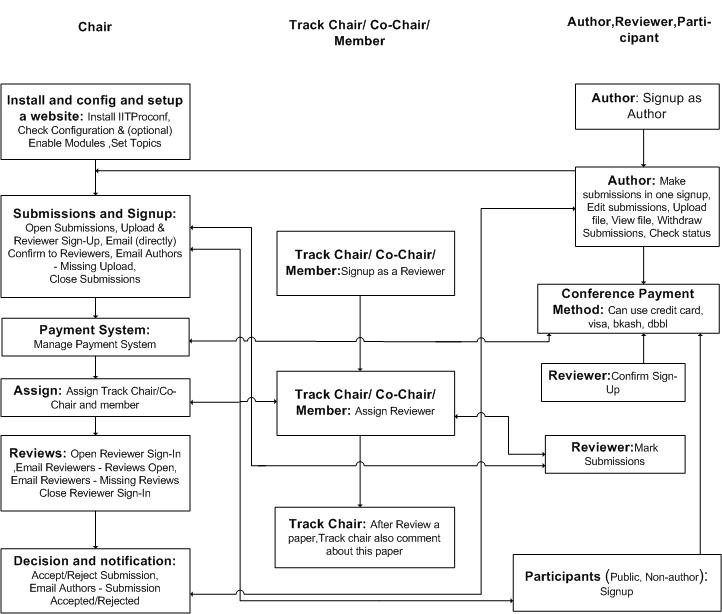
\includegraphics[width=5in]{pic/review}
  \caption{System Overview}\label{system}
\end{figure}


\section{Methodology}

\begin{enumerate}
  \item The research approach try to introduce dataset includes basic requirements of projects with some Functional Measurement types and complexity Factor of the software development effort. So, using dataset for evaluating the proposed model is based on Algorithmic model.
  \item The second attempt will to create an all requirement dataset based on one of requirement, based on model and algorithm.
  \begin{itemize}
    \item Estimate criteria for each requirement in dataset, then asserts it into several equal intervals (lengths).
    \item Cost Factor matrix development
    \item Estimate a corresponding extra linguistic variable for each interval of requirement of Functional Measurement Type.
    \item Estimate Project management software primary functions
  \end{itemize}
\end{enumerate}

\section{Socio-Economic Importance}

\begin{itemize}
  \item Help supervisor to manage resources, control budgets and agenda and develop modern practices.
  \item Help Project Managers to complete on time and within financial plan.
  \item Make better relationship between Software clients and Project Managers \& Developers.
  \item Financial Report generate for Clients satisfaction.
\end{itemize}


\section{Time Frame}

% Please add the following required packages to your document preamble:
% \usepackage{multirow}
% \usepackage[table,xcdraw]{xcolor}
% If you use beamer only pass "xcolor=table" option, i.e. \documentclass[xcolor=table]{beamer}
% \usepackage[normalem]{ulem}
% \useunder{\uline}{\ul}{}
\begin{table}[h!]
\centering
\caption{Time Frame (March 2015 - December 2015)}
\label{time_frame_mar_2015}
\begin{tabular}{|l|l|l|l|l|l|l|l|l|l|l|}
\hline
\multicolumn{1}{|c|}{}                                                                                                             & \multicolumn{10}{c|}{2015}                                                                                                                                                                                                                                                  \\ \cline{2-11}
\multicolumn{1}{|c|}{\multirow{-2}{*}{\textbf{Activity}}}                                                                          & Mar                      & Apr                      & May                      & Jun                      & Jul                      & Aug                      & Sep                      & Oct                      & Nov                      & Dec                      \\ \hline
\multicolumn{11}{|l|}{\cellcolor[HTML]{C0C0C0}\textit{Preparations \& Study}}                                                                                                                                                                                                                                                                                                                                    \\ \hline
\begin{tabular}[c]{@{}l@{}}Activity 1.1 Explore \\ Software Cost And \\ Effort Estimation Models\end{tabular}                      & \cellcolor[HTML]{68CBD0} & \cellcolor[HTML]{68CBD0} &                          &                          &                          &                          &                          &                          &                          &                          \\ \hline
\begin{tabular}[c]{@{}l@{}}Activity 1.2 Development \\ of dataset for \\ Software Cost\end{tabular}                                &                          & \cellcolor[HTML]{68CBD0} & \cellcolor[HTML]{68CBD0} &                          &                          &                          &                          &                          &                          &                          \\ \hline
\begin{tabular}[c]{@{}l@{}}Activity 1.3 Data \\ Collection form \\ Industrial Mentor\end{tabular}                                  &                          &                          & \cellcolor[HTML]{68CBD0} & \cellcolor[HTML]{68CBD0} &                          &                          &                          &                          &                          &                          \\ \hline
\multicolumn{11}{|l|}{\cellcolor[HTML]{C0C0C0}\textit{Development of Approach}}                                                                                                                                                                                                                                                                                                                                  \\ \hline
\begin{tabular}[c]{@{}l@{}}Activity 2.1 Algorithm \\ Development for Actual \\ \& Estimate Software \\ Cost \& Effort\end{tabular} &                          &                          &                          & \cellcolor[HTML]{68CBD0} & \cellcolor[HTML]{68CBD0} & \cellcolor[HTML]{68CBD0} &                          &                          &                          &                          \\ \hline
\begin{tabular}[c]{@{}l@{}}Activity 2.2 Find out \\ Project management \\ software Cost \& Effort\end{tabular}                     &                          &                          &                          &                          &                          & \cellcolor[HTML]{68CBD0} & \cellcolor[HTML]{68CBD0} & \cellcolor[HTML]{68CBD0} &                          &                          \\ \hline
\begin{tabular}[c]{@{}l@{}}Activity 2.3 Differentiate \\ Actual \& Estimated \\ Software Effort and Cost\end{tabular}              &                          &                          &                          &                          &                          &                          &                          & \cellcolor[HTML]{68CBD0} & \cellcolor[HTML]{68CBD0} & \cellcolor[HTML]{68CBD0} \\ \hline
\end{tabular}
\end{table}









% Please add the following required packages to your document preamble:
% \usepackage{multirow}
% \usepackage[table,xcdraw]{xcolor}
% If you use beamer only pass "xcolor=table" option, i.e. \documentclass[xcolor=table]{beamer}
\begin{table}[h!]
\centering
\caption{Time Frame (January 2016 - June 2016)}
\label{time_frame_jan_2016}
\begin{tabular}{|l|l|l|l|l|l|l|}
\hline
\multicolumn{1}{|c|}{}                                                                                                     & \multicolumn{6}{c|}{2016}                                                                                                                                       \\ \cline{2-7}
\multicolumn{1}{|c|}{\multirow{-2}{*}{\textbf{Activity}}}                                                                  & Jan                      & Feb                      & Mar                      & Apr                      & May                      & Jun                      \\ \hline
\multicolumn{7}{|l|}{\cellcolor[HTML]{C0C0C0}\textit{Monitoring and evaluation}}                                                                                                                                                                                                             \\ \hline
\begin{tabular}[c]{@{}l@{}}Activity 3.1 Prepare main \\ case studies to evaluate result\end{tabular}                       & \cellcolor[HTML]{68CBD0} & \cellcolor[HTML]{68CBD0} &                          &                          &                          &                          \\ \hline
\begin{tabular}[c]{@{}l@{}}Activity 3.2 Assessing \\the accuracy of estimates\end{tabular}                              &                          &                          & \cellcolor[HTML]{68CBD0} & \cellcolor[HTML]{68CBD0} & \cellcolor[HTML]{68CBD0} &                          \\ \hline
\begin{tabular}[c]{@{}l@{}}Activity 3.3 Result \\ Analysis \& Report Generate \\ on the basis of Case Studies\end{tabular} &                          &                          &                          &                          & \cellcolor[HTML]{68CBD0} & \cellcolor[HTML]{68CBD0} \\ \hline
\end{tabular}
\end{table}





% \chapter{Literature Survey}
 %\label{chap:Particles}
 %\chapter{System Review}
\section{System Review}

In this arena, some applications are run sequentially. Some of them are – openconf, OCS,OpenWater etc.
Some Modules of this System: Acceptance, Bidding, CAPTCHA, Form Fields, Discussion, File Type, Proceedings.\newline

\textbf{OpenConf:} Install system, check configuration and enable modules, open submission, upload and reviewer signup, assign reviewers and advocates, decision and notification.\newline

In OpenConf, there has no support to create multi-conference system,payment method,Website creation,A/R paper download option,sponsor tracking and speaker schedulingend.

\textbf{OCS(Open Conference System):} Open Conference Systems (OCS) is a free Web publishing tool that will create a complete Web presence for your scholarly conference.OCS will allow you to:create a conference Web site,compose and send a call for papers,electronically accept paper and abstract submissions,allow paper submitters to edit their work,post conference proceedings and papers in a searchable format,post,if you wish,the original data sets,register participants,integrate post-conference online discussions.\newline

In OCS, there has no support to create IEEE eCopyright,Website creation,A/R paper download option,sponsor tracking and speaker scheduling.\newline

\textbf{OpenWater:} OpenWater Conference handles everything, from abstract collection to speaker scheduling, presentation slide management, online registration collection and sponsorship tracking. No matter what you need, you know where to find it.\newline

In OCS, there has no support to create multi-conference system,IEEE eCopyright,payment method,Website creation,A/R paper download option.\newline

Above all systems,there are some advantages and disadvantages.Such as:\newline

\begin{center}
\begin{table}[htbp]
   \begin{tabular}{|c|c|c|c|}
     \hline
     % after \\: \hline or \cline{col1-col2} \cline{col3-col4} ...
     Topics & OpenConf & OCS & OpenWater \\\hline
     Make Submission & Y & Y & Y \\\hline
     Allow Multiconference & N & Y & N \\\hline
     Payment System & In free addition no support & Y & N \\\hline
     Create Website  & N & N & N \\\hline
     P/N Author Registration & N & N & N \\\hline
     IEEE eCopyright & In free addition no support & N & N \\\hline
     A/R paper Download option & N & N & N \\\hline
     Program  Schedule Creation & Y & N & Y \\\hline
     Online Registration & Y & Y & Y \\\hline
     sponsorship tracking & N & N & Y \\
     Make Submission & Y & Y & Y \\\hline
     speaker scheduling & N & N & Y \\\hline
     Program management with RFID & N & N & N \\\hline


   \end{tabular}
   \caption[Pros and Cons Existing System.]{Pros and Cons Existing System}
	\label{tab:pros cons}

  \end{table}
  \end{center}


\section{Proposed  System }
Identify these problems, this proposed system target is to overcome those problems. Primarily, The Proposal entitled as IITProConf can do Peer-Review, Abstract and Conference Management. IITProConf is a free Web publishing tool that will create a complete Web presence for scholarly conference.
IITProconf covers all aspects of online conference management and publishing, from setting up conference website to operational tasks such as submitting, reviewing, editing, publishing, archiving, and indexing of the conference papers.

 IITProconf also helps to manage the people involved in organizing a conference, reviewers, and authors,notifying readers and registrants, and assisting with the correspondence. Additionally, Payment system module is added and free as open source to anyone. In existing all conference system there has no concept of RFID. Main featured of proposed system is helpful to program management with RFID technologies.\newline
Below, there is an overview of the process IITProConf uses.
\begin{center}
\begin{table}[htbp]
   \begin{tabular}{|c|c|c|c|c|c|}
     \hline
     % after \\: \hline or \cline{col1-col2} \cline{col3-col4} ...
     Topics & S/A & Chair & Author & Reviewer & P/N \\\hline
     Install and Config & N & Y & N &N &N \\\hline
     Create Website & N & Y & N &N &N \\\hline
     Open and Close Submissions& Y & N & N &N &N \\\hline
     Sign-Up & N & N & Y &Y &Y \\\hline
     Decision  and Notification & N & Y & N &N &N \\\hline
     Control Conference Payment method & Y & N & N &N &N \\\hline
     Assign  Reviewers & N & Y & N & N & N \\\hline
     Open and close Reviewer Sign-In & N & Y & N & N & N \\\hline
     Review Submission & N & N & N & Y & N \\\hline
     Program management with RFID  & N & Y & N & N & N \\\hline
   \end{tabular}
   \caption[Proposed System Process.]{Proposed System Process}
	\label{tab:system process}

  \end{table}
  \end{center}









%\chapter{System Model}
 \label{chap:Particles}

\chapter{System Process Diagram}




\section{Sequence Diagram}
ProConf helps to manage the people involved in organizing a conference,track chair or co-chair or member,reviewers and authors, notifying readers and registered participants and assisting with the correspondence.In sequence diagram,at first chair create conference website,author signup page,open or close submission,sent email to the people involved in organizing a conference. Author making a submission when chair open submission,upload a file in one account.Track chair assign reviewer,assign paper,gives comment about this paper after reviews.Chair and Track chair or co-chair show all submitted paper.Reviewer reviews paper,give marks assigned paper.Chair accept or reject paper after reviews and sent  notification,email to author.

\begin{figure}[h!]
\centering
  % Requires \usepackage{graphicx}
  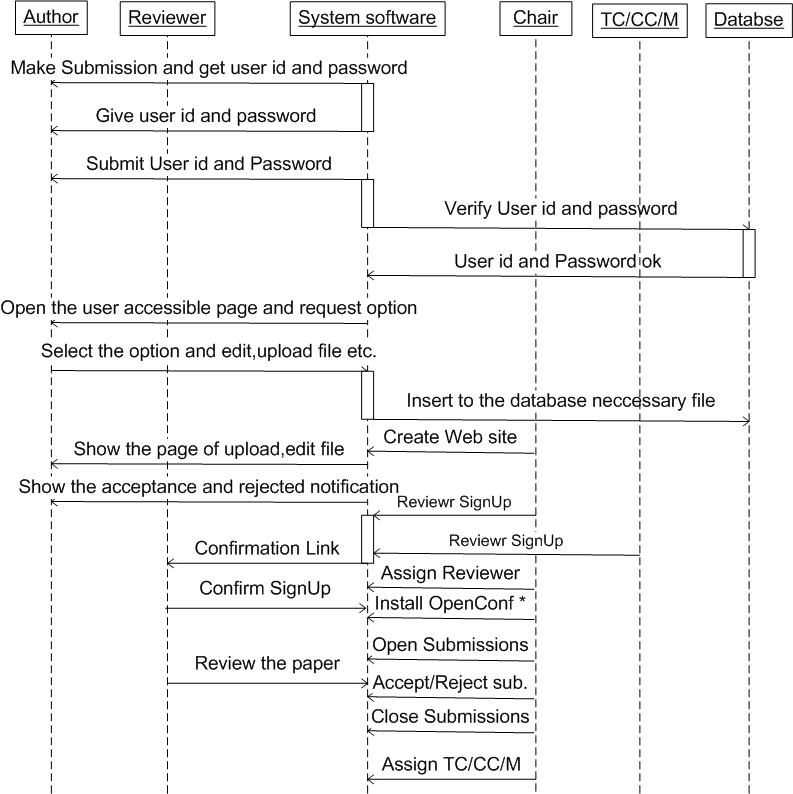
\includegraphics[width=6in,height=3in]{pic/seq1}
   \caption{Sequence Diagram}\label{sequence}
\end{figure}


\section{Activity Diagram}
\subsection{Activity Diagram of Chair’s}
Chair install this system,create conference website,assign reviewer,assign track chair or co-chair or member,accept or reject paper,sent email to the people involved in organizing a conference.

\begin{figure}[h!]
\centering
  % Requires \usepackage{graphicx}
  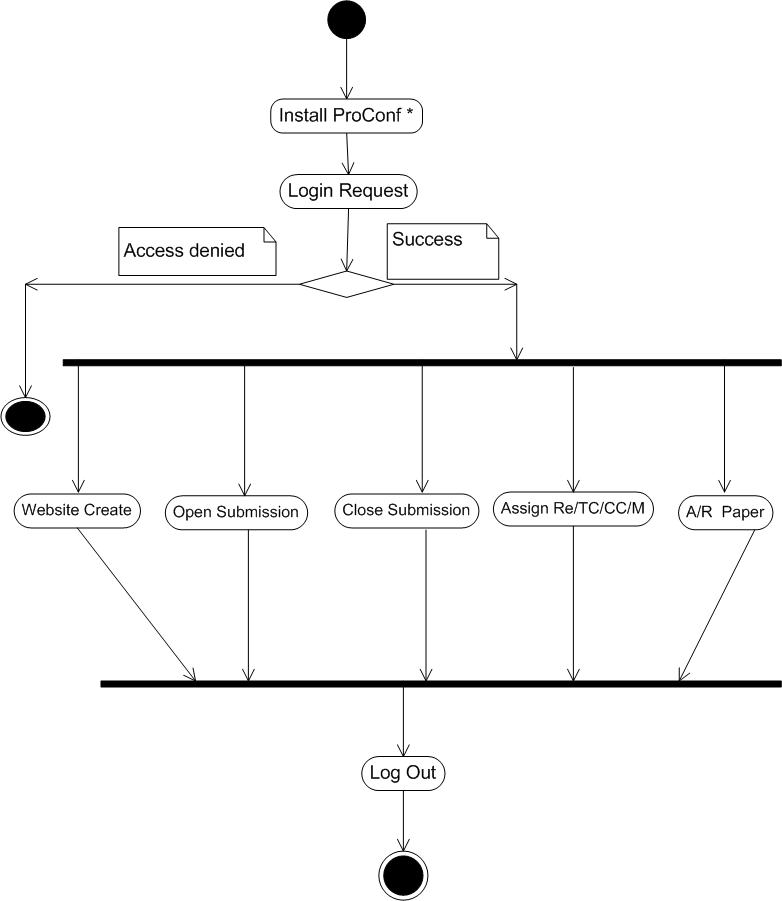
\includegraphics[width=6in,height=6in]{pic/acc}
  \caption{Activity diagram of chair’s}\label{activityc}
\end{figure}
\newpage

\subsection{Activity Diagram of Author’s}
Author making a submission,upload a file,edit file in one account.There will be different color exist to easily identify if file not upload,accept or reject paper,pending paper.
\begin{figure}[h!]
\centering
  % Requires \usepackage{graphicx}
  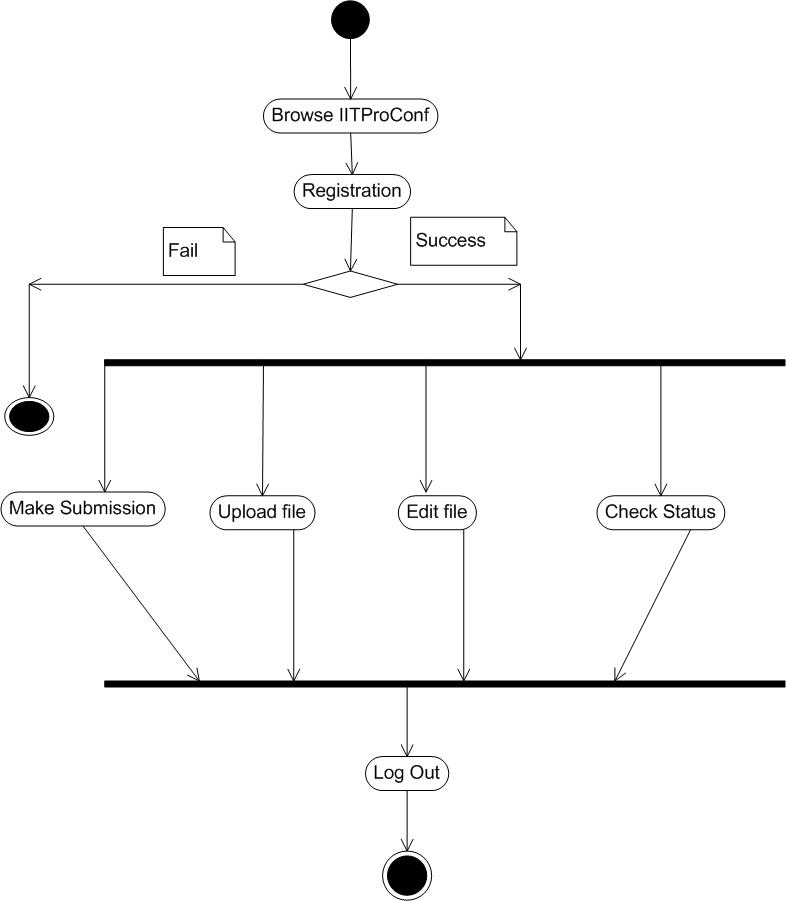
\includegraphics[width=6in,height=7in]{pic/aca}
  \caption{Activity diagram of  author’s}\label{activitya}
\end{figure}

\subsection{Activity Diagram of Track Chair’s or Co-Chair}
Track chair assign reviewer,suggest accept or reject paper,sent email to the people involved in organizing a conference.
\begin{figure}[h!]
\centering
  % Requires \usepackage{graphicx}
  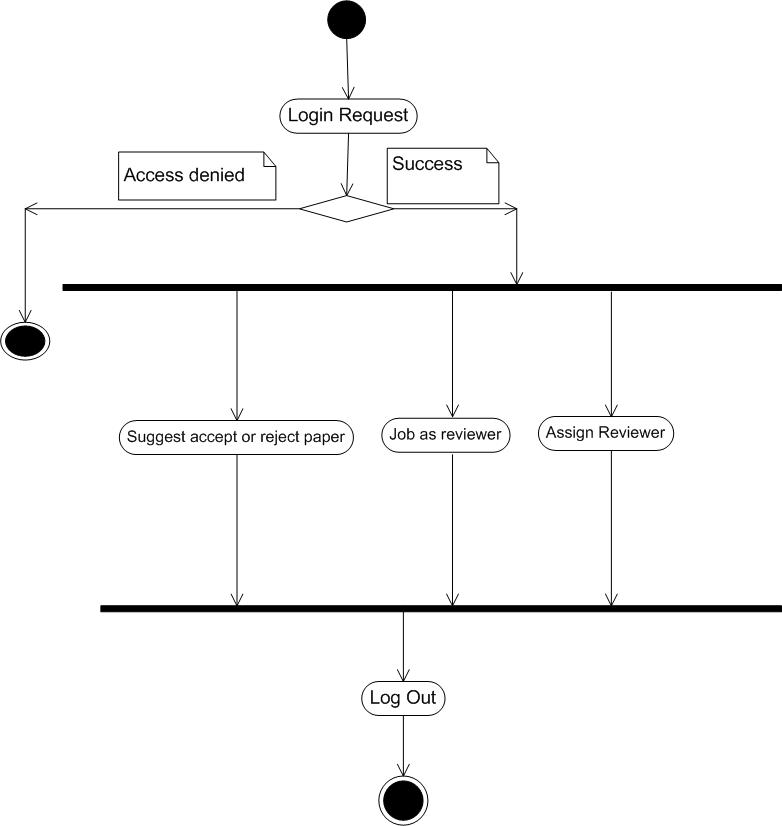
\includegraphics[width=6in,height=7in]{pic/track}
  \caption{Activity diagram of track chair’s or co-chair}\label{activitya}
\end{figure}


\section{Activity Diagram of Reviewer}
Reviewer reviews paper,give marks assigned paper.

\begin{figure}[h!]
\centering
  % Requires \usepackage{graphicx}
  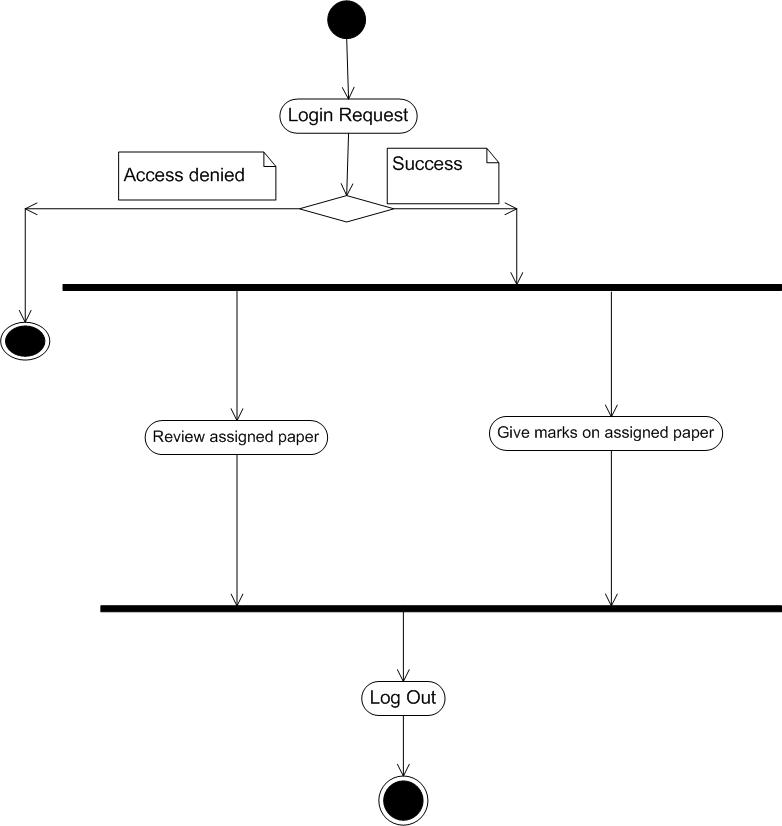
\includegraphics[width=6in,height=7in]{pic/reviewdiagram}
   \caption{Activity Diagram of Reviewer}\label{activityr}
\end{figure}













%\chapter{Simulation Results and Discussion}
 \label{chap:Particles}
 \chapter{Implementation}

\section{Requirements}
The following requirements are applicable if you choose to run ProConf on your own server.

\begin{itemize}
  \item Apache or other* HTTP server
  \item PHP version 5.3.7 or newer, --with-mysqli --with-mcrypt.\cite{ref5}
  \item MySQL or MariaDB version 5 or newer
  \item 15 MB of disk space for the OpenConf software, plus additional space for submission files
  \item	1 MB of database space per 100 submissions (actual amount will vary based on modules installed, number of reviewers, and other factors)
  \item	The hosting account (web server) will also require:
  \item Create/write access to IITProConf/config.php and IITProConf /data/*
  \item MySQL privileges to: ALTER, CREATE, DELETE, DROP, INSERT, SELECT, TRUNCATE, UPDATE
\end{itemize}

\section{Conference Website}
When Chair  install this system then a website will be created.It is easy to use for chair.Chair can create unlimited menu,dynamically news update,change important date etc.All information for conference will be here.Here some option exist that means make submission,scope and track,news,important date,registration,committees,best paper award etc.Conference website will be helpful for authors,reviewer,chair,track chair.


\begin{figure}[h!]
\centering
  % Requires \usepackage{graphicx}
  
\includegraphics[width=5in,height=3in]{pic/all}
   \caption{Conference website}\label{conference}
\end{figure}




\section{Author’s Section}

\subsection{Author make a submission}
In this section author make a submission easily.He/she will make a  unlimited submission in one account.After make a submission, he/she will upload valuable research paper.
\begin{figure}[h!]
\centering
  % Requires \usepackage{graphicx}
  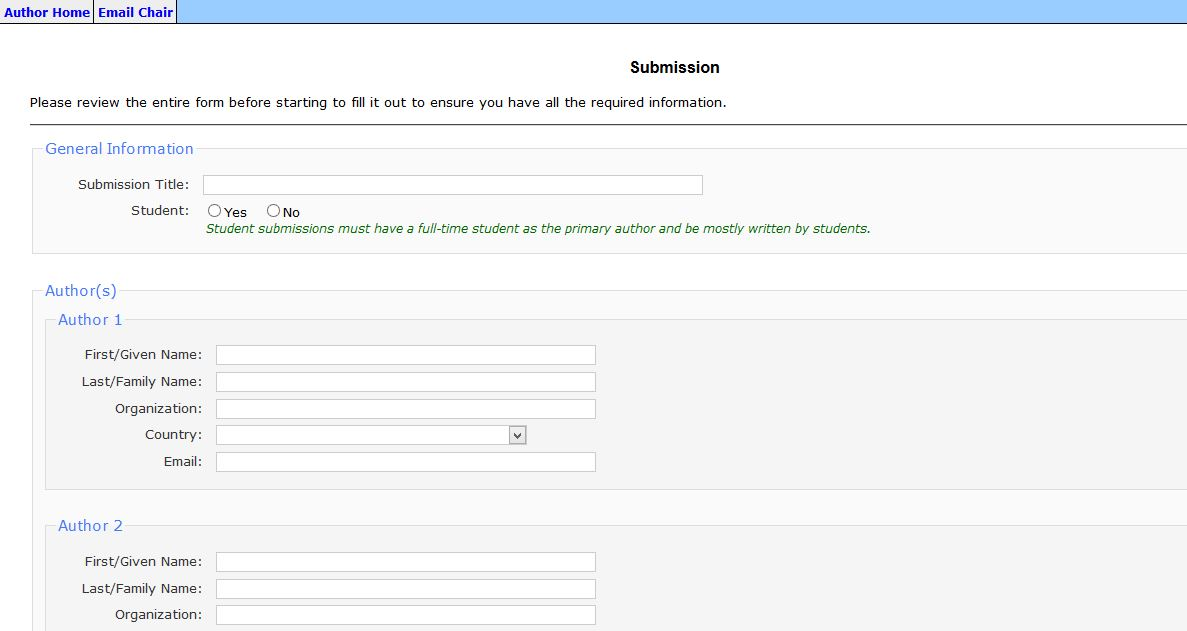
\includegraphics[width=5in,height=3in]{pic/authorm}
   \caption{Author make a submission }\label{authormake}
\end{figure}
\newpage

\subsection{Author home page after submission}
After make a submission then he/she will get a home page.There will be different color exist to easily identify if file not upload,accept or reject paper,pending paper.If chair accept or reject a paper,author will get a notification and a email.If a paper will be accept then author making a camera ready submission.It is very helpful for author for make a submission,upload file,update profile,email chair etc.

\begin{figure}[h!]
\centering
  % Requires \usepackage{graphicx}
  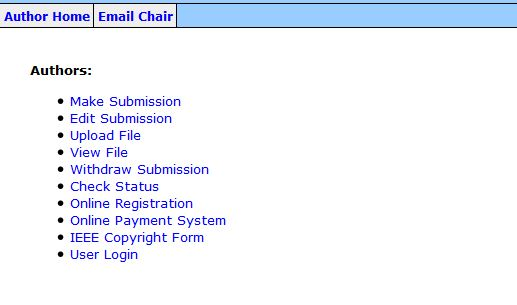
\includegraphics[width=5in]{pic/authorhp}
   \caption{Author home page }\label{authorhome}
\end{figure}



\section{Reviewer home page}
If Chair sign up a reviewer then he/she will get a email for confirmation link.After click a confirmation link as a reviewer,he/she will get a home page.If Chair assign  paper to reviewer,then reviewer will see assign paper.
\begin{figure}[h!]
\centering
  % Requires \usepackage{graphicx}
  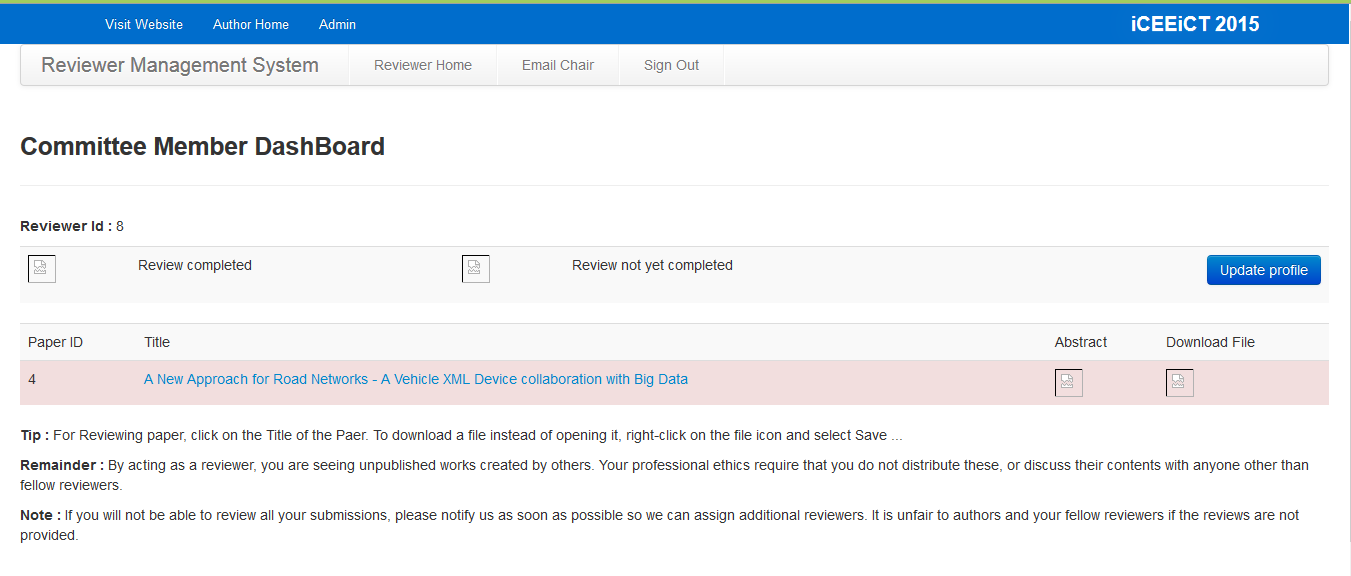
\includegraphics[width=5in]{pic/review1}
   \caption{Reviewer dashboard }\label{review}
\end{figure}



\section{Conference Chair Home Page}
\subsection{Show all paper}
In conference chair home page,chair show the all uploaded paper.There will be different color exist to easily identify if file uploaded or not.

\begin{figure}[h!]
\centering
  % Requires \usepackage{graphicx}
  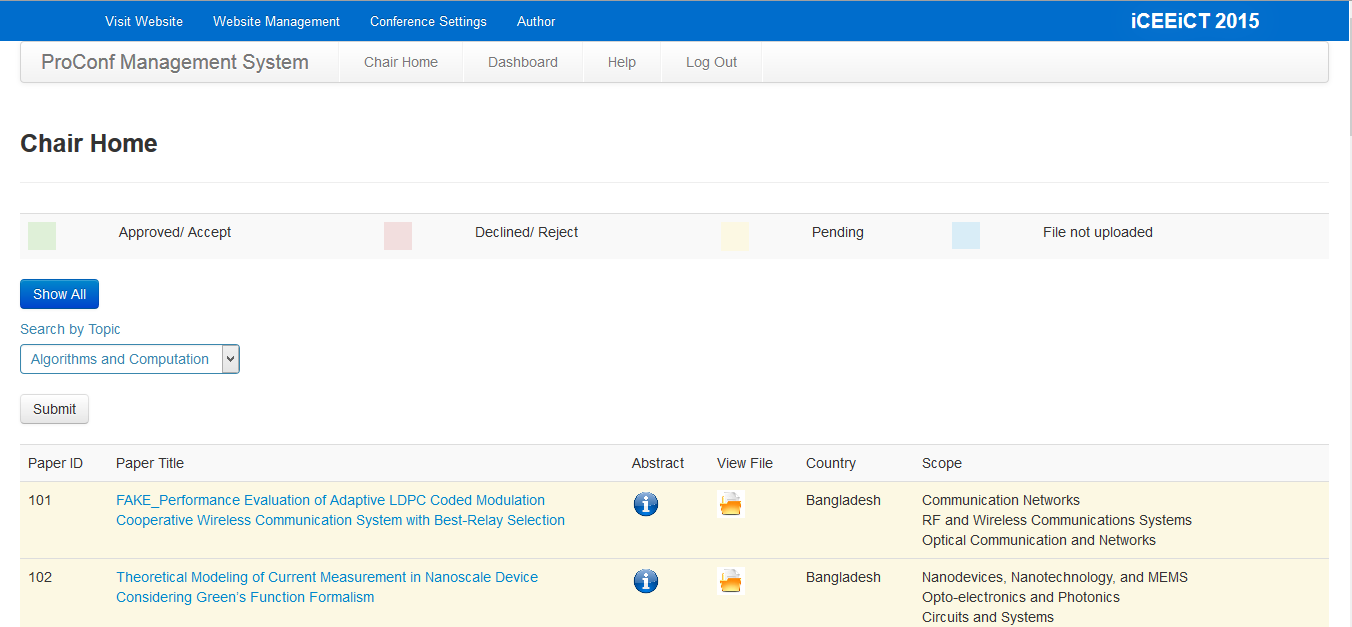
\includegraphics[width=5in,height=2in]{pic/chairhome}
   \caption{Chair home page }\label{chairhome}
\end{figure}


\subsection{ DashBoard}
In conference chair dashboard,chair manage the conference website,pear to pear review system,assign reviewer,accept or reject paper,assign track chair or co-chair or member etc.

\begin{figure}[h!]
\centering
  % Requires \usepackage{graphicx}
  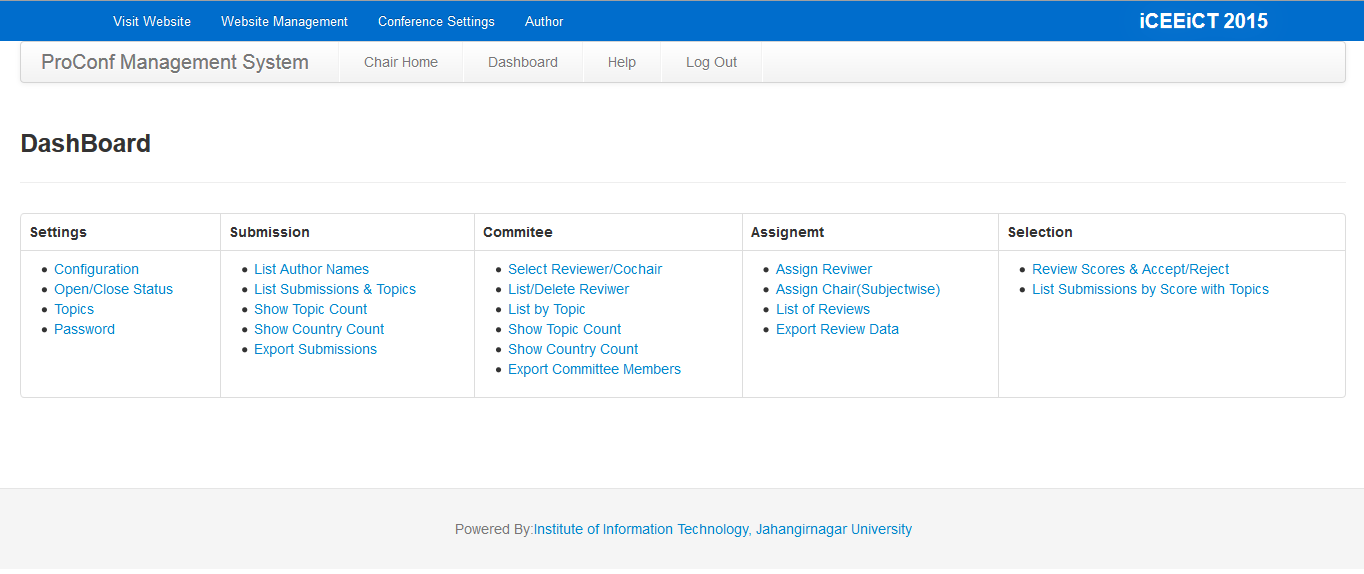
\includegraphics[width=5in]{pic/configuration}
   \caption{Configuration home page }\label{configure}
\end{figure}

\newpage


%\chapter{Conclusion and Future Work}
 \label{chap:conclusion}
 \chapter{Conclusion and Future Plan}
This Thesis will be assessed the structure of research on effort and cost estimation models for web applications by examining the techniques that were castoff to shape approach, the datasets that will  castoff and the research types will be engaged. This will be done in the environment of promoting effort and cost estimation practices from traditional software development.

Although many revisions have been accompanied by effort estimation models for web applications, There is no strong suggestion that there is a certified method or a set of verified approaches for estimating the effort and cost of web applications. All of the performances will be used are tailored forms of systems taken from traditional software engineering.





%\startbibliography
%\begin{singlespace} % Bibliography must be single spaced
 % \bibliography{References.bib}   % Use the BibTeX file ``References.bib''.
%\end{singlespace}
%%\setlinespacing{1.44}
%\bibliographystyle{ieeetr}
% thesis.bbl file edit korte hobe---------------------- reza
\bibliographystyle{plain}
\bibliography{References}
% An external Abstract that can be printed at the end of the document,
% for separate submission to Rackham. Comment it out when not needed. - jg
%\startextabstractpage
%{The Title of Your Dissertation}{Your Name}{Chair: Albert Einstein}
%Software cost models and effort approximations support project supervisors to distribute resources, control budgets
and agenda and develop modern practices, leading to projects completed on time and within financial plan. If cost and effort are determined suspicious in software projects, suitable occasions can be missed; whereas expectant predictions can be affected to some resource losing. In the context of web development, these issues are also vital, and very challenging given that web projects have short schedules and very fluidic opportunity. Since software projects are continually changed in nature, earlier projects may not necessarily cover all aspects of a new project when used
as a basis for cost estimation. Preliminary software estimation models are constructed on regression analysis or mathematical sources. This paper aims to propose an approach to develop the correctness of software effort and cost estimation using the structure of data set of a web application. All the measures collected, apart from total effort, were introduced using the original web hypermedia applications to ensure that functional measurement types were precisely measured. 
%\label{ExtAbstract}

\end{document}
